\section{Experimental setup}

\subsection{Dataset and its Challenges}

The dataset from the SemEval-2025 Task 10, Subtask 2, a task focused on multilingual propaganda narrative detection \cite{semeval2025task10}, spans five languages. While we focus our evaluation on the English subset, our analysis of this task reveals several key characteristics that motivate our architectural choices.

First, the dataset is fundamentally multi-label in nature. A majority of documents (54.0\%) are assigned more than one narrative, with an average of 2.28 labels per document. This necessitates a multi-label modeling approach.

Second, and most critically, the dataset exhibits a severe class imbalance. As shown in Figure~\ref{fig:narrative_distribution}, the 22 narrative labels follow a classic long-tailed distribution. The most frequent narrative appears 65 times more often than the least frequent one. This sparsity poses a significant challenge for traditional supervised models, which risk overfitting on the few ``head'' classes and failing to generalize to the many rare but meaningful ``tail'' classes. This characteristic strongly motivates our adoption of a zero-shot paradigm, which does not depend on label frequencies in a training set.

\begin{figure*}[!ht]
\centering
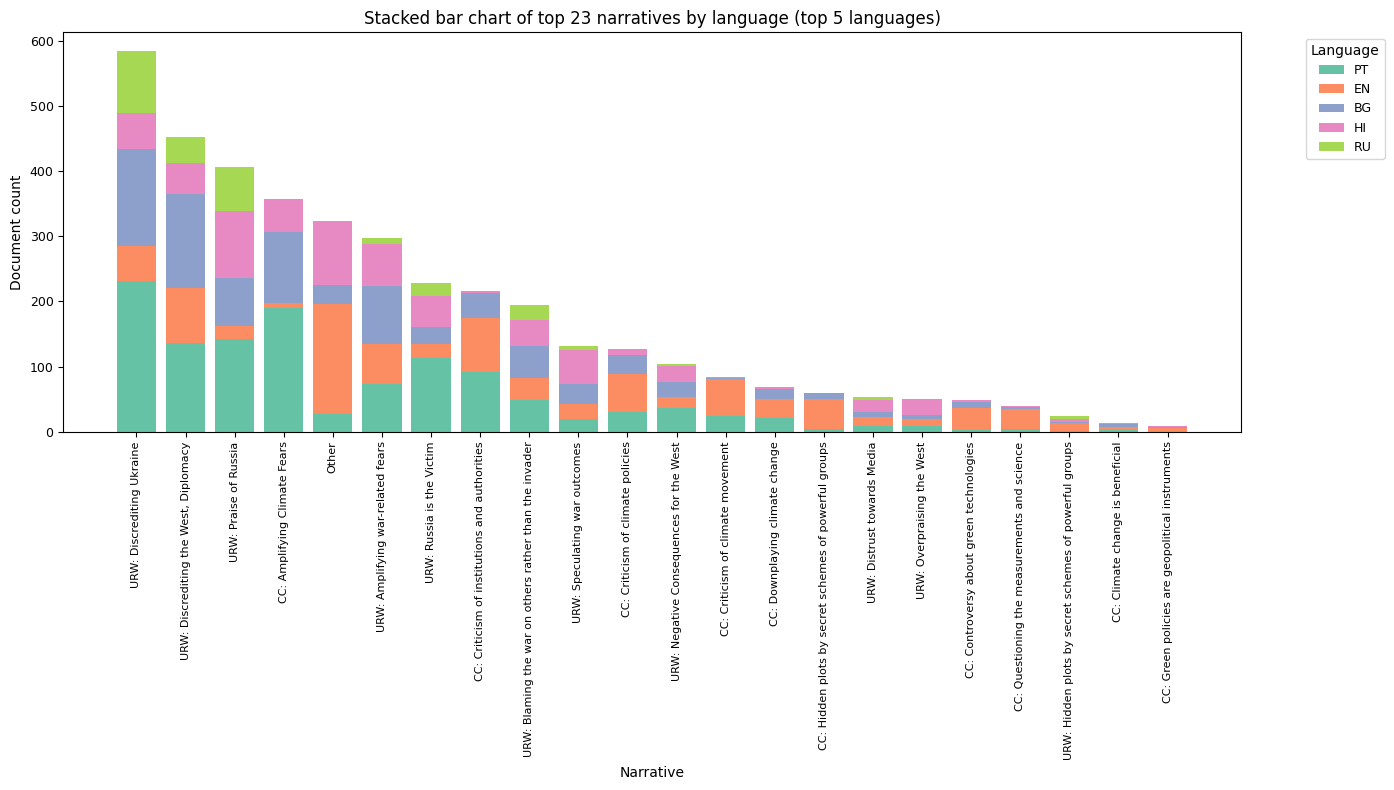
\includegraphics[width=0.95\textwidth]{assets/images/data_description/narrative_distribution.png}
\caption{Long-tailed distribution of narrative labels. A small number of frequent narratives dominate the dataset, while most are rare. This severe imbalance justifies the use of zero-shot LLM approaches that do not rely on large per-class training counts.}
\label{fig:narrative_distribution}
\end{figure*}

Due to the multi-label nature and severe class imbalance inherent in the dataset, we decided to adopt a zero-shot learning approach. This paradigm avoids dependency on large per-class training counts and is well-suited to handle the long-tail distribution of narratives, making it ideal for this challenging classification task.

\subsection{Hardware Configuration}

All experiments were conducted on a machine with the following specifications:
\begin{itemize}
\item \textbf{Processor:} Intel Core 9 Ultra
\item \textbf{GPU:} NVIDIA RTX 4070 (8GB VRAM)
\item \textbf{Memory:} 32GB RAM
\item \textbf{Storage:} 1TB SSD
\end{itemize}

\subsection{Evaluation Scope}

We primarily evaluate the performance of our models on the English test set, providing detailed analysis and interpretation of the results on this language. However, to assess the multilingual capabilities of our approaches, we also conducted experiments on additional languages to validate the generalizability of our methods across different linguistic contexts.